%%%%%%%%%%%%%%%%%%%%%%%%%%%%%%%%%%%%%%%%%%%%%%%%%%%%%%%%%%%%%%%%%%%
%                                                                 %
%                            CHAPTER FOUR                         %
%                                                                 %
%%%%%%%%%%%%%%%%%%%%%%%%%%%%%%%%%%%%%%%%%%%%%%%%%%%%%%%%%%%%%%%%%%%

\chapter{RESULTS}\label{ch:implement}

\section{DATASETS INTRODUCTION}

\subsection{Noble Gas Dataset}

The ``Global Database on \textsuperscript{3}He/\textsuperscript{4}He in on-shore free-circulated subsurface fluids" is a tumultuous database \cite{Polyak2015}.
The first version, published in June 11, 2013, contains 8 files with 194 columns each.
The next version of the database, published March 8, 2015, compiles all the data into a single file and reduces the number of columns to 54, marking a drastic change.
In addition, several columns changed the units with which they reported measurements.
While usage documentation, explaining the content and use of the data, accompanied each version, no records were included indicating what changed between versions.
A change log would be valuable guide with such drastic structural and content changes.
The third and most recent publication came in July 11, 2017, with no changes to the number of files or columns, but many new rows.

\subsection{Copper Dataset}

The Paragenetic Mode for Copper Minerals database became available through collaboration with the author's lab to create new methods of visualizing mineralogy relationships \cite{Morrison2016}.
The first version was collected June 8, 2016, with the update following soon after on August 8, 2016.
Major edits are fairly limited with only 16 column additions and 2 removals between the versions.
Value formats remain consistent from one version to the next, resulting in a much more condensed body of changes, making transitions more easily verifiable.
Compared to the Noble Gas data set, it provides a more stable data platform to implement the versioning model in Chapter \ref{ch:model}.
The data from this work is also more processing friendly, making it agreeable to automatic change log generation.

\subsection{GCMD Keywords}

The Global Change Master Directory (GCMD) is a metadata repository used by NASA to store records of its available data sets \cite{Miled:2001:GCM:372202.372324}.
They employ a set of keywords to make NASA Earth Science data sets searchable.
These words tag and label datasets into strictly defined categories \cite{GCMDKey}.
GCMD Keywords do not qualify as a standard web ontology since it does not constitute a class hierarchy.
The management team stored early versions of the keywords in Excel spreadsheets, and a centralized distribution system was not used until June 12, 2012.
The Key Management Service now serves the keywords directly in a variety of formats.
Each version of the keywords, encoded in RDF, were downloaded into separate files.
Only versions from June 12, 2012 and after were available, resulting in 9 version files.
Each keyword corresponds to a unique identifier, and when combined with a web namespace, resolves to a data description of the keyword.
Every identifier can be referred to per version by including the version's number at the web identifier's end, meaning that identifiers are consistent across versions.
The taxonomy uses the concepts \textit{skos:Broader} and \textit{skos:Narrower}, where skos refers to the Simple Knowledge Organization System ontology name space, to form a tree hierarchy \cite{skos}.
The tree's root is the keyword, "Science Keywords."
The data set provides an interesting study case due its long sequence of versions and ready use of linked data technology \cite{Stevens2016}.

\begin{table}
	\caption{List of versions available in the KMS.}
	\label{gcmd_table}
	\centering
	\begin{tabular}{|c|c|c|c|c|c|c|c|c|}
		\hline
		June 12, 2012 & 7.0 & 8.0 & 8.1 & 8.2 & 8.3 & 8.4 & 8.4.1 & 8.5 \\
		\hline
	\end{tabular}
\end{table}

\subsection{MBVL Classifications} \label{sec:MBVL}

The Marine Biodiversity Virtual Laboratory (MBVL), based at Woods Hole Oceanographic Institution, provides data and services for the study of marine biology with an integrative approach \cite{mbvl}.
In the application studied, a choice of algorithm and taxonomy pairings must be tested on a known population in order to estimate their performance with an unknown microbial population.
The original sequences belong only to the species listed in Table \ref{species_table}.
However, this data is not available to the author, and only the list of species are known, forming the first data set in this section.
These sequences are then grouped and classified by a specific taxonomy and algorithm pairing.
The workflow utilizes two taxonomies, the Ribosomal Database Project (RDP) and the Silva taxonomy.
Using these databases, the Species-level IdentificatioN of metaGenOmic amplicons (SPINGO) or the Global Alignment for Sequence Taxonomy (GAST) algorithms assign taxonomic ranks to each sequence.
This produces four data sets, each using the same grouping identifiers and having the same size in each group.
This means that the only difference between the data sets are the ranks assigned to each group.

\begin{table}
	\caption{List of species in the original population.}
	\label{species_table}
	\centering
	\setlength{\tabcolsep}{2pt}
	\begin{tabular}{|c|c|c|}
		\hline
		Acinetobacter baumannii & Actinomyces odontolyticus & Bacillus cereus \\
		Bacteroides vulgatus & Clostridium beijerinckii & Deinococcus radiodurans \\
		Enterococcus faecalis & Escherichia coli & Helicobacter pylori \\
		Lactobacillus gasseri & Listeria monocytogenes & Neisseria meningitidis\\
		Porphyromonas gingivalis & Propionibacterium acnes & Pseudomonas aeruginosa \\
		Rhodobacter sphaeroides & Staphylococcus aureus & Staphylococcus epidermidis\\
		Streptococcus agalactiae & Streptococcus mutans & Streptococcus pneumoniae \\
		\hline
	\end{tabular}
\end{table}

\section{Creating a Versioning Graph}

The Noble Gas and Copper data set authors assert that the files in each set are versions of each other.
We can also verify they are versions by taking a look at their provenance.
For the Copper data set, the objects result from a compilation effort with the same sources of data.
An entry recording the source material for each row in the table accompanies each reading.
As a result, these entries were used to determine that they share similar provenance.
They will also both be used as data inputs at the same step to generate data visualizations.
By considering the related provenance and workflow involvement, we can surmise that the files are different \textbf{manifestations} of the same \textbf{work}.
Determining whether the Noble Gas files are versions is a more challenging activity.
From provenance graphs like the one constructed for the entry CAM001 in Figure \ref{CAM001ProvGraph}, the entries share a common source document.
Likewise, a significant portion of the other entries also share sources from the same body of work.
The ones that do not are new or removed entries.
As there was no personal involvement in the use of this data set, determining whether they can occupy the same workflow step requires actually looking into the files.
\begin{figure}
	\centering
	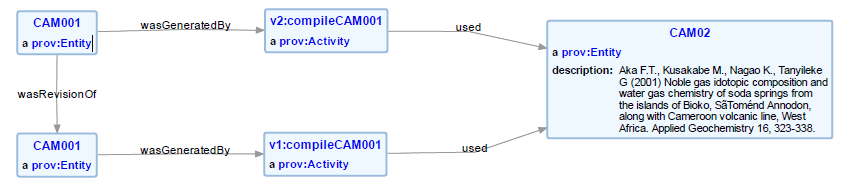
\includegraphics[scale=0.70]{figures/CAM001v1v2.png}
	\caption{Provenance graph for the CAM001 entry of the Noble Gas Database.  Other than the labels, the structure of each data object is very much the same.}
	\label{CAM001ProvGraph}
\end{figure}
Investigating column headers and the accompanying documentation reveals that they report many of the same measurements.
Some amount of leeway is given in this assessment as having every quantity match would mean that the two files aren't versions, but the same object.
This process helps to determine the confidence that using the model to encode the discovered changes will result in a meaningful versioning graph.


\subsection{Form a Mapping} \label{mapping}

The next step involves formulating a method to determine whether a relationship constitutes an add, invalidate, or modify mapping.
As discussed in the previous chapter, this relies on determining whether an attribute exists in one version, the other, or both.
However, with tabular data, a row and column attribute is required to match specific cells.
For the Noble Gas data set, this is the entry identifier and the column headers.
Row and column numbers are avoided because edits can result in the same entry associated with different indices.
In addition, the first version of the Noble Gas data set was organized into multiple files so the same row index would appear more than once, and therefore, could not be used to match related entries.
An observation that also simplifies identifying edits is that cells are rarely added or removed individually.
When one row gains a cell all other rows gain one as well, perhaps with null values, forming a new column.
As a result, data additions and invalidations only use one identifier.
A basic method to determine the identifiers involved in an addition is straight forward.
A set of identifiers \(\mathcal{A} = \mathcal{R}_{r} - \mathcal{R}_{l}\) where \(\mathcal{R}_{l}\) and \(\mathcal{R}_{r}\) correspond to the row identifiers of the left-hand and right-hand versions, respectively.
A converse procedure reveals the set of invalidated attributes \(\mathcal{I} = \mathcal{R}_{l} - \mathcal{R}_{r}\).
All the remaining identifiers exist in both versions and form a set of possible modification attributes.
These are only possibilities because the mapping procedure does not check for differences, and as a result, rows that have not undergone a change are also included.
The same is done with columns.
This only performs a very basic version mapping, but data producers can significantly improve this with their more intimate understanding of the versions.
For example, the base method would not understand that a Location column has been divided into two columns Latitude and Longitude.
A data producer could manually link the Location attribute to the Latitude and Longitude attributes, forming a single modification instead of an invalidate and two additions.

The Copper Minerals data set starts each row with a unique mineral name, which can be matched across data sets to determine if an entry has undergone a modification.
The column headers have different formats because the initial file is an Excel file and the other is a comma separated file.
As a result, the column headers were manually matched together with the remaining headers in each file mapped into the added and invalidated sets.
The Noble Gas database also uses unique identifiers to mark each of its entries, but the first version of the database divides data among multiple files.
For this reason, the identifiers must first be collected into a single dictionary data structure mapping identifiers to their files.
The version map is then computed from this data structure.
The database also uses multi-line headers which makes a basic automated approach difficult since the cells are not well aligned.
This means that the columns for this database also had to be mapped manually to find the matching columns.

\subsection{Produce Change Log}

While a linked data versioning graph can now be generated using the mapping method, it is difficult to visualize without using more specialized software.
The solution is to create a human readable change log to both validate the mapping matches and generate human readable change documentation.
This addresses a gap in the Noble Gas data set's documentation which describes data use, but not data changes.
The log is divided into three sections corresponding to the sets generated in Section \ref{mapping}.
However, this provides an opportunity to address a weakness in modern change logs in that they are only human readable.
Two technologies previously introduced, RDFa and JSON-LD, provide a means of embedding linked data into HTML documents, allowing the log to be both human and machine readable.

\begin{figure}
	\centering
	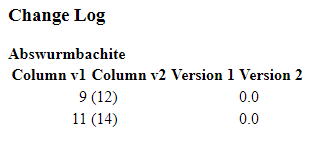
\includegraphics[scale=0.80]{figures/Changelog-zoomed.png}
	\caption{Abswurmbachite entry in the Copper Dataset Change Log}
	\label{changelog_zoomed}
\end{figure}

Consider the entry in Figure \ref{changelog_zoomed} from a change log of the Copper data set.
RDFa uses the attributes in HTML documents to include linked data describing content on the page.
This means that an automated web agent can read the document and extract the associated versioning graph.
A selection of the marked up source from Figure \ref{changelog_zoomed} appears in Listing \ref{rdfa_list}.
Only the lines displaying table headers and the second data line have been removed.
Immediately, it can be seen that the markup is quite cluttered as a result of the clash between RDFa's intent and its use.
The goal of this technology is to describe the content on a page and give context to particular values, marking a string of digits as a phone number for example.
However, in this application, very little of the content is used in the model except for line 3, which uses the mineral name as an attribute label.
It is instead used to encode the versioning model into the HTML document's lattice, leveraging the ability to imply relationships in nested tags.
Unfortunately, RDFa interpreters are very particular in the way they resolve implications, and the order in which data appears in a change log to be human readable does not match the order they need to be for RDFa to encode the model.
In lines 10 and 11, two triples have to be explicitly included in order to conform with the model outlined in Chapter \ref{ch:model}.

\begin{lstlisting}[language=HTML, caption=Abswurmbachite RDFa, label=rdfa_list]
<h3>Change Log</h3>
<div about="Version1" rel="vo:hasAttribute">
  <div resource="v2:Abswurmbachite" typeof="vo:Attribute">
    <span style="font-weight:bold" property="http://www.w3.org/2000/01/rdf-schema#label">Abswurmbachite</span>
    <table rel="vo:Undergoes">
      <tr  about="ChangeAbswurmbachite12" typeof="vo:Change">
        <td align="right" rev="vo:Undergoes" resource="v1:AttributeAbswurmbachite12v1" typeof="vo:Attribute"> 9</td>
        <td property="vo:resultsIn" resource="v2:AttributeAbswurmbachite12v2" typeof="vo:Attribute">(12)</td>
        <td>          </td>
        <td>       0.0</td>
        <span about="Version1" property="vo:hasAttribute" resource="v1:AttributeAbswurmbachite12v1"></span>
        <span about="Version2" property="vo:hasAttribute" resource="v2:AttributeAbswurmbachite12v2"></span>
      </tr>
    </table></div></div><br>
\end{lstlisting}

The difficulties adopting RDFa into the change log arise from a misalignment in intent and use.
Alternatively, a technology meant to store data in web documents, such as JSON-LD, may produce better results.
Listing \ref{json_list} provides the alternative encoding of the Abswurmbachite entry from RDFa.
While significantly longer, the number of triples is not limited by the tag count within a change.
It also separates the human-readable content from the model data, making the source easier to code and modify.
Additionally, a decision was made to divide each change's linked data into its associated row instead of collecting them all at the bottom or top of the page in a single script node.
The practice of a one-node collection is generally helpful for many web applications to load data quickly, but since this is not an application, it makes more sense to break up the content.
Changes to individual attributes can be identified using anchors on the web page, then agents need only extract and parse the link data to these specific entries.
This way, a subgraph of only the pertinent attributes can be created without first ingesting the entire versioning graph.
However, a problem both of these change logs struggle with is size.
The Copper Minerals data set encoded in RDFa is 1.7 MB and JSON-LD is 3.3 MB.
In the Noble Gas data set, the RDFa and JSON-LD change log sizes are 59 and 60 MB, respectively.
The Noble Gas change logs often do not load in a browser.

\begin{lstlisting}[language=HTML, caption=Abswurmbachite JSON-LD, label=json_list]
<h3>Change Log</h3>
<div about="v1:Abswurmbachite">
  <span style="font-weight:bold" property="http://www.w3.org/2000/01/rdf-schema#label">Abswurmbachite</span>
  <table>
    <tr  id="ModifyChangeAbswurmbachite12">
      <td align="right"> 9</td>
      <td >(12)</td>
      <td>          </td>
      <td>       0.0</td>
      <script type="application/ld+json">
[
{
	"@context": "https://orion.tw.rpi.edu/~blee/provdist/GCMD/VO.jsonld", 
	"@id": "http://CUdb.com/v1/AttributeAbswurmbachite9", 
	"@reverse": {
		"hasAttribute": "Version1"
	}, 
	"@type": "vo:Attribute", 
	"label": "Primary", 
	"undergoes": "http://orion.tw.rpi.edu/~blee/provdist/CU/DTDI/CUjsonlog.html#ModifyChangeAbswurmbachite12"
}, 
{
	"@context": "https://orion.tw.rpi.edu/~blee/provdist/GCMD/VO.jsonld", 
	"@id": "http://orion.tw.rpi.edu/~blee/provdist/CU/DTDI/CUjsonlog.html#ModifyChangeAbswurmbachite12", 
	"@type": "vo:ModifyChange", 
	"resultsIn": "http://CUdb.com/v2/AttributeAbswurmbachite12"
}, 
{
	"@context": "https://orion.tw.rpi.edu/~blee/provdist/GCMD/VO.jsonld", 
	"@id": "http://CUdb.com/v2/AttributeAbswurmbachite12", 
	"@reverse": {
		"hasAttribute": "Version2"
	}, 
	"@type": "vo:Attribute", 
	"label": "Primary"
}
]
      </script>
    </tr>
  </table></div><br>
\end{lstlisting}

\subsection{Generate Versioning Graph}

A versioning graph is now generated using the mapping method determined in Section \ref{mapping}.
Since the attributes in sets \(\mathcal{A}\) and \(\mathcal{I}\) guarantee a change, each item is encoded into linked data and output to a document.

\begin{lstlisting}[language=SPARQL, caption=Noble Gas Add in Turtle, label=NGA]
<http://rdfa.info/play/Version1> a vo:Version ;
	vo:absentFrom <http://rdfa.info/play/AddChange21> .
<http://rdfa.info/play/AddChange21> a <https://orion.tw.rpi.edu/~blee/VersionOntology.owl#AddChange> ;
	vo:resultsIn <http://rdfa.info/play/Attribute21> .
<http://rdfa.info/play/Attribute21> a <https://orion.tw.rpi.edu/~blee/VersionOntology.owl#Attribute> ;
	rdfs:label "EGY001"
<http://rdfa.info/play/Version2> a vo:Version ;
	vo:hasAttribute <http://rdfa.info/play/Attribute21>
\end{lstlisting}
Listing \ref{NGA} presents the statements in turtle format necessary to express that the entry EGY001 has been added to the data set from Version 1 to Version 2 as shown in Figure \ref{NobleGraph1}.
Notice that the namespace for many of the URIs is \textlangle http://rdfa.info/play/\textrangle.
This results from the triples being extracted out of an HTML change log with embedded linked data, and this is used as the default namespace for the page.
Since we know the number of additions, each change instance can be easily numbered.
Add changes are also kept separate to allow for individual annotation.
Likewise, the graph generator iterates over the set of invalidations and generates a set of statements to instantiate each invalidate change.

\begin{figure}[b]
	\centering
	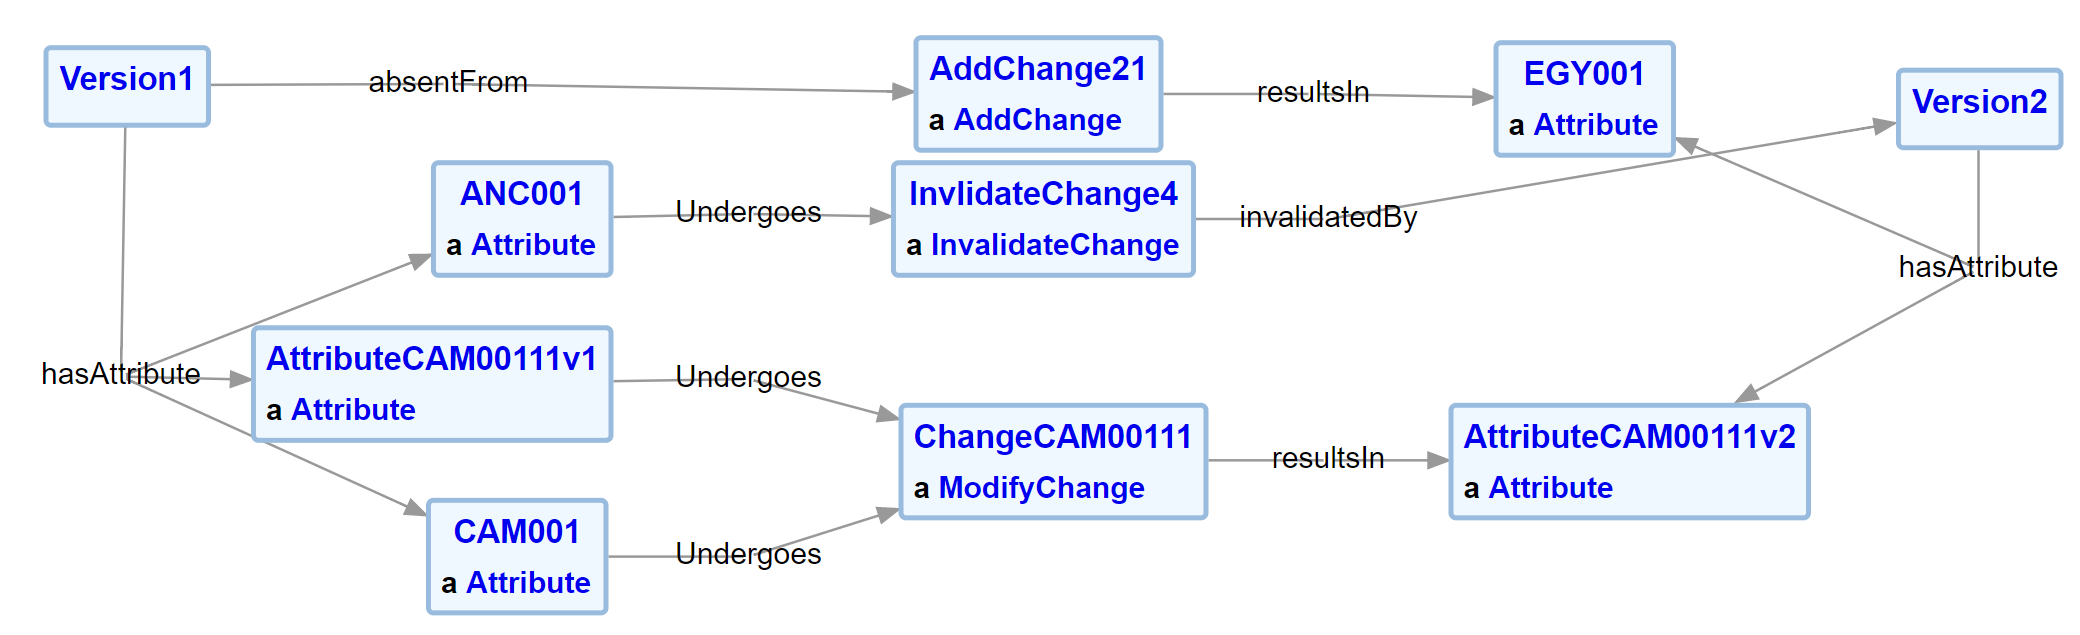
\includegraphics[scale=0.30]{figures/NobleVersion.png}
	\caption{Some initial entries from versions 1 and 2 of the Noble Gas data set}
	\label{NobleGraph1}
\end{figure}

However, Figure \ref{NobleGraph1} also demonstrates an interesting set of decisions made early in the generation process regarding modifications.
Firstly, the relation presented in the figure is unbalanced and the right-hand side of ChangeCAM00111 links only to the column identifier but not to the corresponding row attribute.
This links from a mismatch between the model's structure, the order in which data appears in the change log, and the way RDFa links properties together.
Because the row label forms the outermost encapsulation, it cannot instantiate both row identifiers and implicitly link them separately.
To do so would require explicitly instantiating the attribute in a non-visible part of the document which would defeat the purpose of using RDFa to implicitly encode the versioning graph into the document.
Secondly, the column identifier AttributeCAM00111v1 combines together the row label and the column number, making it unique to just the CAM001 row.
This was a decision to properly identify the attribute as it appears in the change log document.
Since the item is not a generic column 11 element in the log, but a specific item of CAM001, the entry id is included in the column identifier.
This formulation poses a problem when trying to query the graph and determine how many rows have a column 11 modify change for example.
When the versioning triples are not extracted from a change log and printed as linked data, the structure has greater freedom as seen in Figure \ref{NobleGraph2}.

\begin{figure}
	\centering
	\begin{adjustbox}{addcode={\begin{minipage}{\width}}{
					\caption{Versioning Graph representing the linked data graph with selected entries of additions, invalidations, and modifications. 
			}\end{minipage}},rotate=90,center}
		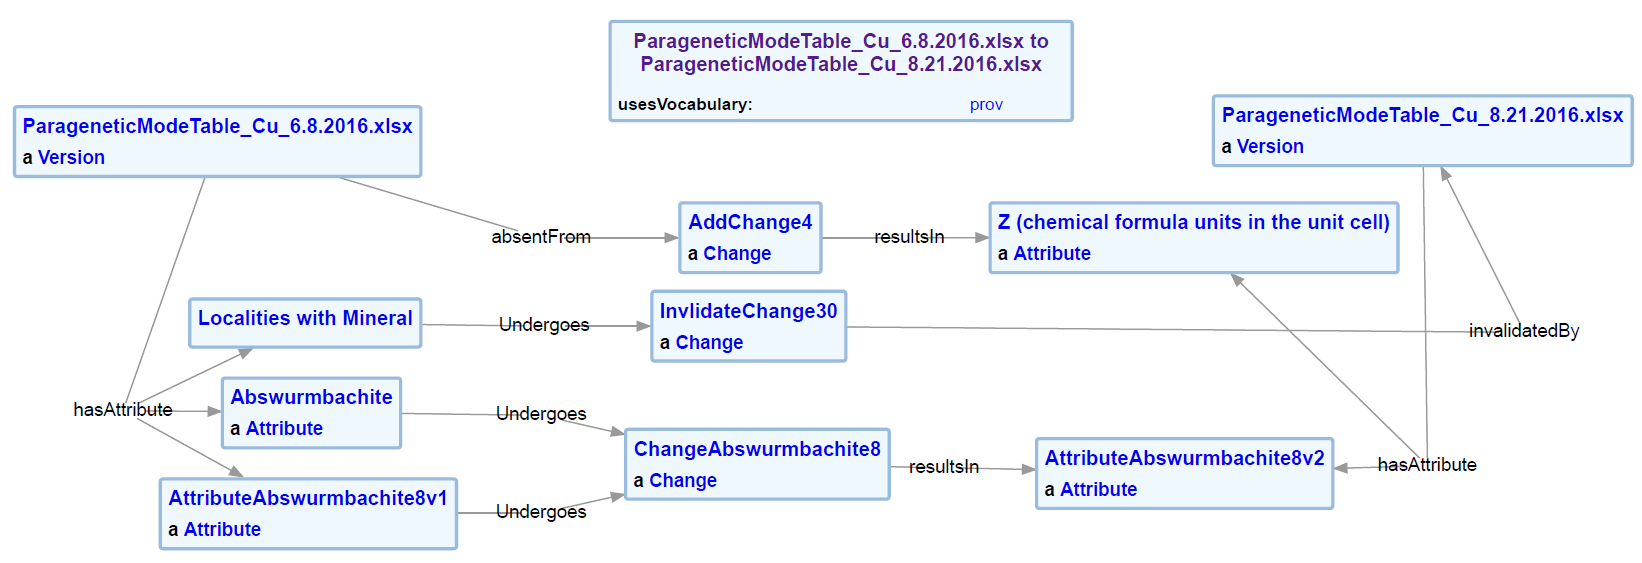
\includegraphics[scale=0.5]{figures/VersioningGraph2.png}%
	\end{adjustbox}
	\label{CopperGraphVerGraph}
\end{figure}

\subsection{Graphs with Multiple Versions}

Figures \ref{NobleGraph1} and \ref{CopperGraphVerGraph} depict a comparison between only two versions, but a project can contain more than two objects.
Case in point, a third version of the Noble Gas data set was released on July 11, 2017.
Figure \ref{NobleGraph2} shows a subgraph that contains changes from all three versions of the Noble Gas data set.
From the first to second version of the data, EGY001 becomes introduced as an attribute into the data set.
This entry then undergoes a modification change in columns 29, 31, and 43 when comparing versions two and three.
Entry TUR030 goes through a modification change in column 11 from version one to version two.
The entire row, however, becomes invalidated in version three.

\begin{figure}
	\centering
	\begin{adjustbox}{addcode={\begin{minipage}{\width}}{
					\caption{Versioning Graph representing the linked data graph with selected entries of additions, invalidations, and modifications after the publication of the third version. 
			}\end{minipage}},rotate=90,center}
		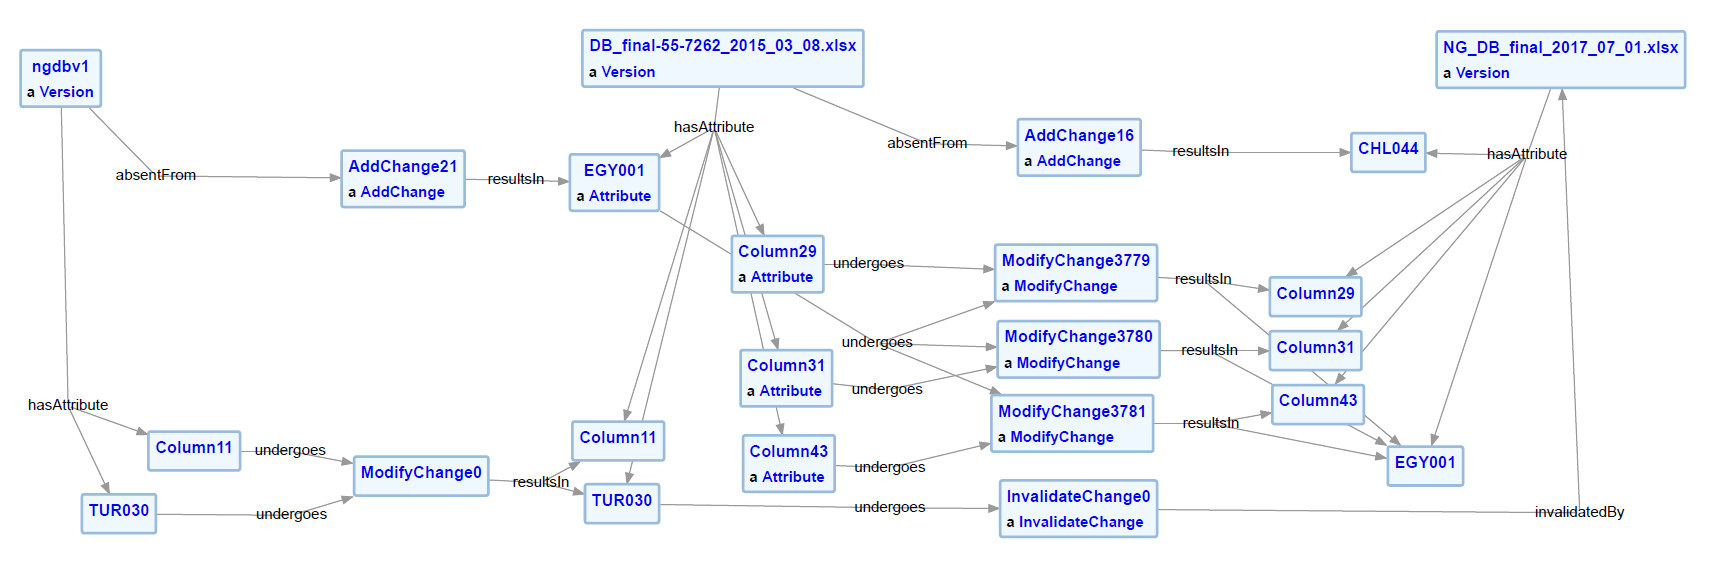
\includegraphics[scale=0.5]{figures/NobleVersion2.png}%
	\end{adjustbox}
	\label{NobleGraph2}
\end{figure}

Notice the difference in how Figure \ref{NobleGraph1} and Figure \ref{NobleGraph2} refer to columns.
Figure \ref{NobleGraph1} used linked data extracted from a change log employing RDFa, forcing the row identifier and the column identifier into the same concept.
The way nesting works in RDFa means that ChangeCAM00111 cannot back reference multiple concepts in a single statement, therefore AttributeCAM00111v2 was used to imply CAM001.
Figure \ref{NobleGraph2} used linked data extracted from a JSON-LD encoded change log.
Since the log can use explicit statements, the column identifier refers to the entire column and can be used to identifier changes in the same column across multiple rows.

\section{GCMD}

\subsection{Creating the Versioning Graph}

The Global Change Master Directory maintains and releases the different versions of their keyword list.
From this, it can be concluded that each edition shares provenance and can be used in the same workflow step.
This conclusion is further justified as each keyword concept uses the same Unique Resource Identifier (URI) across versions.
The identifiers also act as an ideal key in the version mapping.
While additions and invalidations are simple to identify using these keys, modifications are not since a change in the key would result in completely different object.
Instead, we look at the immediately broader concept.
Each keyword uses the concepts \textit{skos:Broader} and \textit{skos:Narrower}, where skos refers to the Simple Knowledge Organization System ontology name space, to form a tree hierarchy with the broadest concept "Science Keywords" forming the root.
A modification would then result if a concept moved to a different place in the hierarchy.
This would result in the removal of a child node from the parent and a different broader concept for the child, meaning two modifications occur.
However, in this project, only the child is recorded since it is the concept that moves around in the hierarchy.
Versioning graphs for each comparison was generated by extracting JSON-LD from the corresponding change log, and entering the triples into a Fuseki triple store.

\subsection{Quantifying Change}

The GCMD group migrated their keywords into a centralized Keyword Management System (KMS) as of June 12, 2012.
Each subsequent keyword release has been supplied an identifier by the management group and the add, invalidate, and modify counts between each transition are presented in Figure \ref{GCMDC1}.
The query used to extract the counts is found in Listing \ref{gcmd_list}.
Notice the sharp spike in adds and invalidates when transitioning from version 8.4.1 to 8.5.
Not only should a small transition not produce changes of this magnitude, but the data sets size is on the order of the recorded invalidates.
In addition, no modifications are revealed, and even the root node "Science Keywords" has been invalidated.
Further investigation of the root word reveals that the name space for the keywords has changed from HTTP to HTTPS.
Since the identifiers are unique, this means they no longer refer to the same object after the protocol change.
This results in the whole data set being invalidated and a new data set being added.
However, the dot decimal identifier only indicates a minor change, demonstrating a difference between the producer's perceived divergence and the actual change.
To provide context, NASA mandated a transition to secure protocols, and the group changed the named space to ensure the URIs remained resolvable.

\begin{figure}%[b]
	\centering
	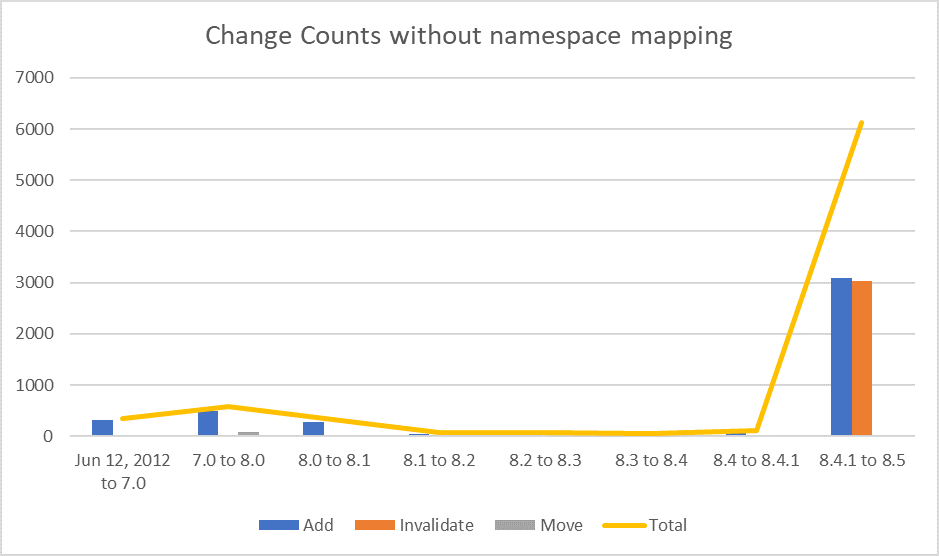
\includegraphics[scale=1]{figures/GCMDChart1.png}
	\caption{Add, Invalidate, and Modify counts in Version 8.5.  The counts show change magnitudes and indicate that major and minor changes differ by orders of magnitude.}
	\label{GCMDC1}
\end{figure}

%\hfill \break
\begin{lstlisting}[language=SPARQL, caption=This query compiles the counts for each subclass of Change in a GCMD versioning graph,label=gcmd_list]
PREFIX vo:<http://orion.tw.rpi.edu/~blee/VersionOntology.owl>
PREFIX rdfs:<http://www.w3.org/2000/01/rdf-schema#>

SELECT ?p (COUNT (DISTINCT ?s) as ?count)
{
?s a ?p .
?p rdfs:subClassOf vo:Change .
} GROUP BY ?p
\end{lstlisting}

That the data producers did not perceive this change in name space to be a major modification can be demonstrated by accounting for the change and recounting.
In the modified mapping, HTTP and HTTPS identifiers are treated the same.
Differences in change magnitudes become much clearer after controlling for the altered name space in Figure \ref{GCMDC2}.
All revisions are dominated by additions, but major version changes have counts around 300 to 500 while minor revisions are an order of magnitude smaller.
This includes the transition from version 8.4.1 to 8.5.
From the identifier scheme and the change counts, it is clear that the keyword management team expected only minor changes in the keywords.
This analysis demonstrates that relying on data producers to name their versions using the dot decimal identifiers based on their perceived change also relies on their perceiving the intended utilization of their data set by all their users.
The count results seem to indicate that they can differentiate between major and minor revisions, but it also shows that current version labels may not capture all the change within a transition.


\begin{figure}%[b]
	\centering
	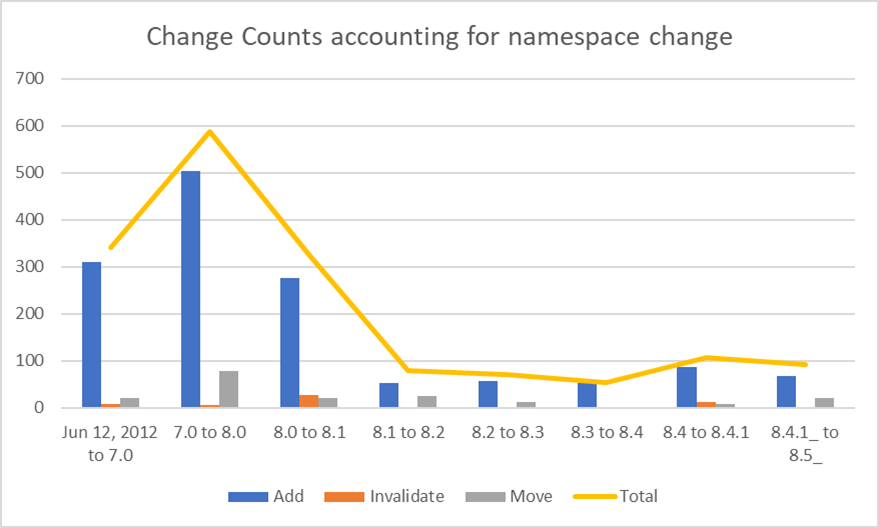
\includegraphics[scale=1]{figures/GCMDChart2.png}
	\caption{Add, Invalidate, and Modify counts ignoring the namespace changes in Version 8.5.  The counts show change magnitudes appropriate for the identifier.}
	\label{GCMDC2}
\end{figure}

\section{MBVL}


The goal of this section is to use the versioning graph to compare the accuracy of different algorithm and taxonomy combinations in determining the taxonomic classification of marine microbiological species.

\subsection{Versioning Graph}

The experiment undergoes two phases of comparison in this procedure.
The first phase compares the initial species content with the classifications by a particular algorithm/taxonomy combination.
Since the classification results from a population selected according to the initial species list, these two data sets share a common provenance.
However, the list cannot be used in place of the classifier results because not only does it have only 21 entries, but also it does not have a clear correspondence with the DNA chains sent to the classifier.
As a result, these two sets are not versions of each other, and versioning results will have weak implications.
A labeling of the initial input data, could be considered a version of the results, but that data product is not available.

Each taxonomy and classifier combination outputs a taxonomic classification for each entry from the same source.
Shared input data indicates the results share common provenance.
The classifications also share the same workflow step because their results have similar formats, reporting a specific taxonomic name for each entry.
Since classifications occur over the same set of entries, their identifiers can be used to match outputs together for comparison.
However, if this method of matching is used, every mapping would be a modification since each identifier appears in all data sets, and it would not provide any comparison based on the algorithm's specificity.
Instead, a mapping using the accuracy of each algorithm is used.
Since a name is assigned at a taxonomic rank to a sequence only if it passes the algorithm's confidence level, matches can be determined on whether a classifier can confidently decide more or fewer ranks.
As a result, additions and invalidations ascertain whether a classifier can identify more or less of an entry's taxonomic name while modifications indicate the same specificity but mismatching names.
This method of mapping versions allows the results to give insight into the accuracy of different algorithm and taxonomy combinations.